\subsection{O1: the K\"ohler camera-shake benchmark}
\label{sec:kohler}
The benchmark~\cite{kohler2012} contains 48 photographs (4 scenes $\times$ 12 recorded hand-shake
trajectories replayed on a robot) with sharp frames along each trajectory. Reference kernels were
obtained by regularised Fourier division of each blurred image by a sharp frame; restoring with
them gives the ceiling. Ground truth for scenes 2 and 3 could not be retrieved in full (the archived
download is truncated), so PSNR is reported on the 24 images of scenes 1 and 4, following the
benchmark protocol (best PSNR over the sharp frames after intensity scaling and registration);
kernel comparisons use all 48 images.

\begin{figure}[h]
\centering
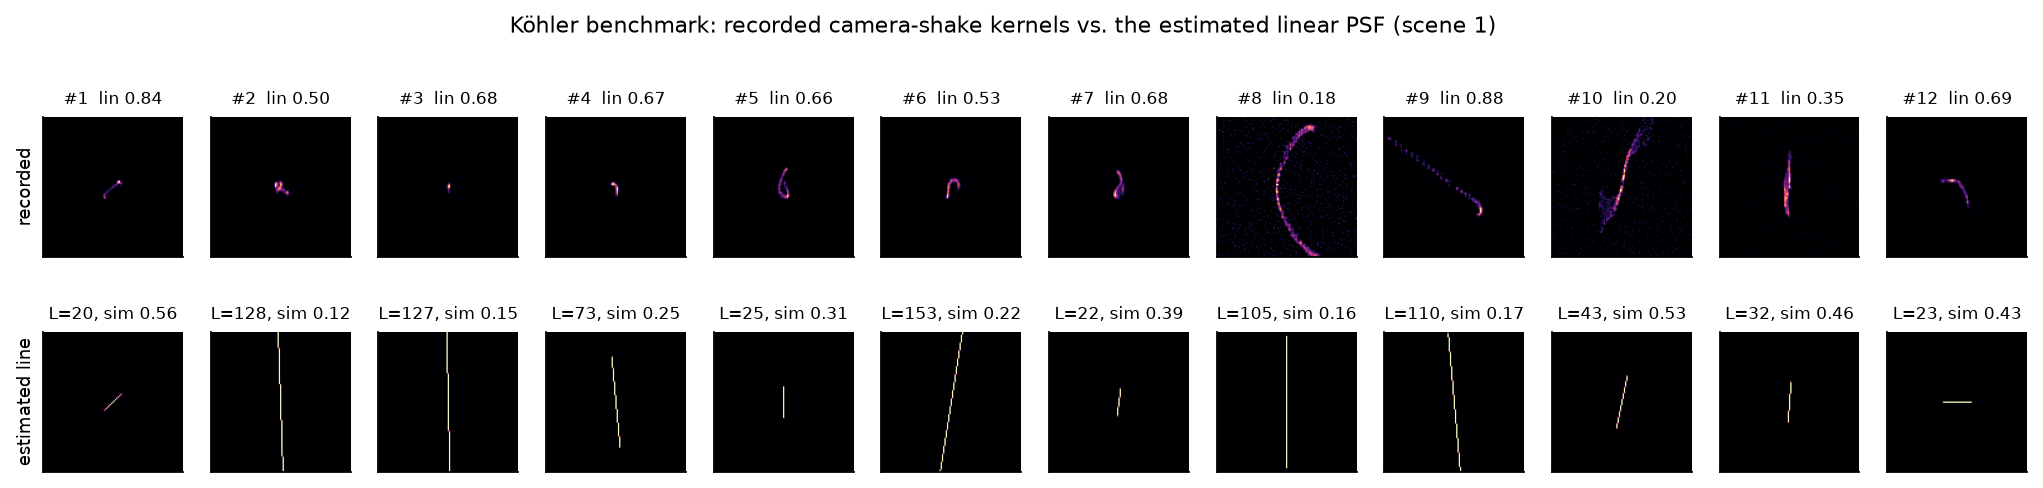
\includegraphics[width=\textwidth]{06_kohler_kernels.png}
\caption{Recorded camera-shake kernels (top, with a linearity score from second moments: 1 = straight
line) and the estimated line kernels (bottom; $L$ and cosine similarity to the recorded kernel).}
\label{fig:kohlerk}
\end{figure}

\begin{table}[h]
\centering\small
\begin{tabular}{lc}
\toprule
restoration (RL, 60 iterations, discrepancy stopping) & benchmark PSNR (dB), 24 images \\
\midrule
blurred input & 24.39 \\
recorded (reference) kernel --- ceiling & \textbf{29.24} \\
best straight-line fit to the recorded kernel & 23.42 \\
baseline estimate & 20.44 \\
text-aware estimate & 20.42 \\
text-aware estimate + gate (62\% accepted) & 24.08 \\
\bottomrule
\end{tabular}
\caption{K\"ohler benchmark.}
\label{tab:kohler}
\end{table}

\begin{figure}[h]
\centering
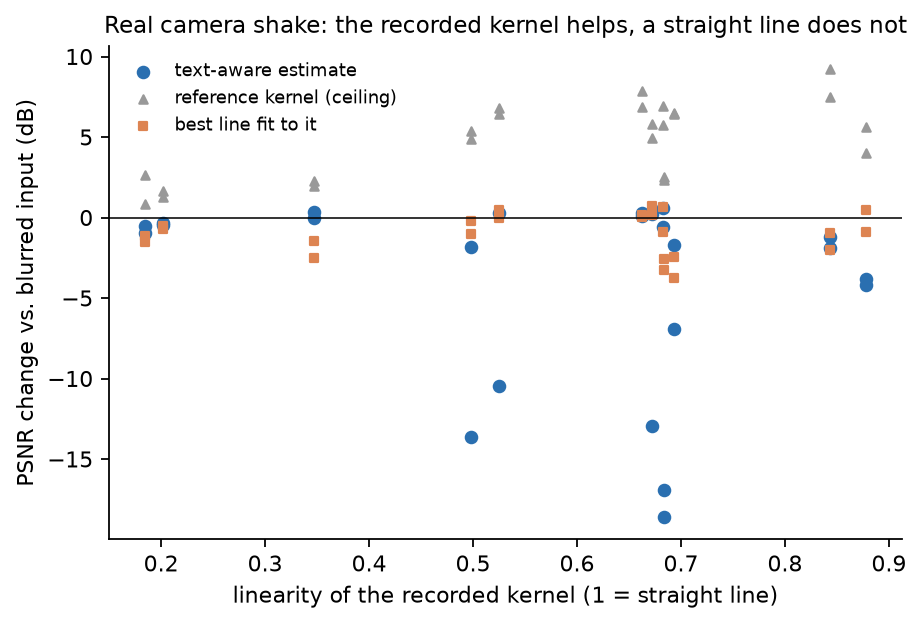
\includegraphics[width=0.6\textwidth]{06_kohler_gain_vs_linearity.png}
\caption{PSNR change against the blurred input versus how straight the recorded trajectory is.}
\label{fig:kohlerg}
\end{figure}

\paragraph{Findings.} Real hand shake is not a straight line (Fig.~\ref{fig:kohlerk}): only 2 of the
12 trajectories have a linearity above 0.75, and most are hooks and arcs. The consequence is
decisive: even the \emph{best} line kernel fitted to the recorded kernel loses 1\,dB against the
blurred input, while the recorded kernel gains 4.9\,dB. So the limiting factor on this benchmark is
the uniform-line model itself, which the proposal fixed as the scope, rather than the estimator. The
estimated lines are further off (75\% of restorations are worse than the input). On the two
near-linear trajectories the text-aware estimate finds the angle within $10^\circ$ in half the images,
against 38\% for the baseline. The gate helps less here than on plates: it accepts 15 of the 24
images and 9 of those restorations still hurt, because a curved trajectory still gives a strong,
consistent dominant direction in every image half. Detecting \emph{model} failure of this kind needs
a test of the line hypothesis itself (e.g.\ comparing the dip pattern with that of the fitted line),
which we leave as future work.
